\chapter{Introduction} 

\section{Livestock farming, animal health and infectious diseases}

% [\textcolor{red}{A update une fois que j'aurai fini cette section}]
Livestock farming today is embedded in a complex socio-economic landscape that underpins food security, rural development, and environmental sustainability. As global populations rise and resource constraints become more acute, the ability to produce high-quality animal products in a sustainable manner is more critical than ever. This sector not only ensures the availability of nutritious food but also supports the livelihoods of countless rural communities, thereby reinforcing local economies. In parallel, the modern challenges of animal health and public safety are converging, with infectious diseases emerging as a significant threat that jeopardizes both the productivity of farming systems and the broader public health framework. The traditional approach to livestock management, which often treats animal health in isolation, is increasingly being questioned in favour of a more integrated strategy that acknowledges the intricate links between animal welfare, human well-being, and environmental health.

In this context, infectious diseases are not merely biological phenomena but are embedded within the socio-economic fabric of livestock farming. Their impact reverberates through production losses, escalating veterinary expenses, and the overuse of antibiotics, which in turn contribute to public health concerns such as antimicrobial resistance. These challenges demand a rethinking of conventional control measures and underscore the urgency of developing sustainable farming practices that can adapt to both immediate crises and long-term environmental pressures. By embracing an integrated approach, the sector can transform these challenges into opportunities for innovation, leveraging advanced technologies and interdisciplinary strategies to enhance animal health, protect public well-being, and ensure the economic viability of farming systems for future generations.

This section provides a comprehensive overview of the socio-economic landscape that surrounds livestock farming, underscoring its importance for food security, public health, environmental management, and the integrated “One Welfare” approach. It section also highlights key challenges related to the impact of infectious diseases on livestock farming as well as conventional methods used to diagnose, manage, and prevent these diseases and their inherent limitations.

\subsection{Socio-economical context and the stakes}



% Finally, the rationale for integrating new, data-driven modelling approaches is introduced, emphasizing their potential to improve disease surveillance and decision-making. These methods aim to complement the expertise of farmers and veterinarians by providing more accurate prognostics, optimizing resource use, and ultimately contributing to more resilient and welfare-focused livestock farming systems.

\subsubsection{Livestock Farming, animal health well-being}

Livestock farming constitutes a cornerstone of global agriculture, underpinning food security and rural development while driving significant economic contributions worldwide (Fig \ref{fig:chap1-livestock}). In Europe, the average livestock farm covers approximately 34 hectares and maintains a herd size of around 47 livestock units, a scale that reflects both intensive production and resource management practices \cite{INRA_Livestock_Production}. Globally, the sector contributes up to 50\% of the agricultural gross domestic product and supports the livelihoods and food security of nearly 1.3 billion people in developing countries, highlighting its critical role in sustaining rural economies \cite{Herrero2016, FAO2017}

The environmental footprint of livestock farming is also considerable. Livestock production occupies nearly 75\% of the agricultural land, underscoring its extensive spatial demands and the pressure it exerts on natural ecosystems \cite{Steinfeld181371}. High animal densities in confined feeding operations lead to substantial nutrient emissions, with studies reporting significant releases of nitrogen and phosphorus into the environment, thereby contributing to issues such as greenhouse gas emissions and water eutrophication \cite{Ramankutty2018, Mallin2015, LI2016451}


\begin{figure}[h]
  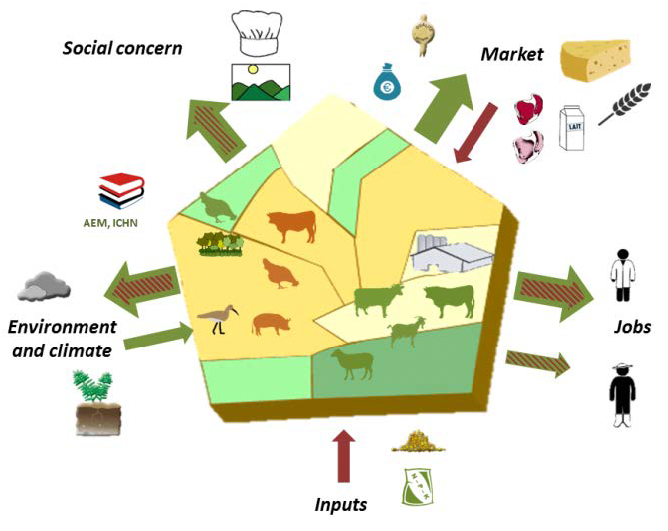
\includegraphics[width=\linewidth]{figures/chap1/chap1-livestockfarming.png}
  \caption{Bundle of services in areas with both crop and livestock farming. Illustration from \cite{INRA_Livestock_Production}}
  \label{fig:chap1-livestock}
\end{figure}

Future projections indicate a continuing rise in global demand for animal products, a trend driven by the so-called "livestock revolution" that accompanies increasing incomes and population growth, particularly in emerging economies \cite{Delgado2016}. This anticipated growth in demand is set against the backdrop of an already extensive current offer, where production scales and market dynamics are closely intertwined. Furthermore, livestock production accounts for about 15\% of global greenhouse gas emissions, with ruminants being the primary contributors due to their lower feed conversion efficiencies \cite{Gerber2013}. These figures underscore the urgency of balancing the expanding demand with sustainable production practices that safeguard both environmental quality and public health.

Animal health and welfare remain central to the sustainability of livestock farming systems. Societal concerns over animal well-being are driven not only by ethical considerations but also by the direct links between robust animal health, food safety, and public health outcomes. Ensuring high standards of animal welfare enhances productivity by improving feed conversion efficiency and reducing culling rates, while also reinforcing consumer trust in the safety and quality of animal products \cite{FAO2017}.

One of the major pressures on livestock farming is infectious diseases. These diseases challenge animal health and welfare, threaten food security and public health, and raise ecological concerns. The following subsection provides a brief overview of infectious diseases, detailing their intricate relationship with the environment and their overall impact on livestock systems.


\subsubsection{Livestock infectious diseases}

Bernard Vallat, Director General of the World Organisation for Animal Health (OIE), emphasized the escalating challenges posed by infectious diseases by stating, “As a result of globalisation and climate change, we are currently facing an unprecedented worldwide impact of emerging and re-emerging animal diseases and zoonoses (animal diseases transmissible to humans)” \cite{vallat2007protecting}. Indeed, infectious diseases represent a significant threat to livestock farming, deeply intertwined with environmental, economic, and public health factors. These diseases are caused by pathogenic microorganisms including bacteria, viruses, fungi, and parasites, capable of spreading directly or indirectly among animals, across species barriers (zoonoses), or through contaminated environmental media such as soil, water, or feed. Infectious disease has been chosen for consideration because globally these diseases have historically been, continue to be, and are expected to remain major concerns in the future. The increasing intensification of modern animal husbandry has encouraged the proliferation of infectious diseases and resulted in the emergence and increased importance of so-called multifactorial diseases.

Within livestock systems, infectious diseases manifest in diverse forms and can be categorized by their clinical presentations and modes of transmission. Respiratory infectious diseases, notably bovine respiratory disease complex and contagious bovine pleuropneumonia, pose substantial threats due to their rapid spread and significant economic impacts. Gastrointestinal infections such as salmonellosis and coccidiosis critically impair animal health and productivity through severe digestive disruptions. Bloodstream infections, exemplified by African swine fever, are particularly devastating due to their rapid progression, high mortality rates, and significant implications for international trade. Vector-borne diseases like bluetongue, transmitted by biting midges, are increasingly problematic in regions experiencing climate change, altering vector habitats and expanding disease ranges. Skin infections, including dermatophytosis and footrot, impose chronic health and welfare issues, severely affecting productivity and animal product quality \cite{gilbert2024quantifying}

The economic repercussions of infectious diseases in livestock are substantial, with diseases such as African swine fever and bovine tuberculosis significantly reducing productivity and incurring considerable veterinary costs \cite{gilbert2024quantifying}. Moreover, globalization, climate variability, and intensive farming practices further facilitate pathogen proliferation and dissemination, amplifying the scale and severity of outbreaks. Historical translocation events have dramatically demonstrated this potential, with diseases such as rinderpest and foot-and-mouth disease causing severe disruptions to global livestock production and trade \cite{GUMMOW201041}. Additionally, the widespread emergence of antibiotic resistance, driven by excessive antibiotic use in animal agriculture, poses critical challenges to effective disease management, raising serious concerns for animal welfare and health due to therapeutic failures \cite{bengtsson2014antibiotic}. To mitigate these threats, conventional control measures have and still play a employed, which are explored in the following subsection.


\subsection{Conventional control strategies of infectious diseases}
\label{Conventional control strategies} % ajout-du-label-pour-faire-reference-a-la-sous-section

Conventional control strategies for managing infectious diseases in livestock primarily rely on accurate diagnosis and prognosis to mitigate outbreaks and prevent their spread. Diagnosis involves identifying diseases through clinical appraisal, visual and tactile assessments conducted by farmers and veterinarians—and biological examinations, including laboratory analyses like PCR tests on collected samples. Prognosis entails predicting the potential progression and impact of identified diseases based on expert knowledge, historical data, and empirical observations. These methods culminate in tailored control recommendations, such as vaccination, quarantine, biosecurity protocols, and prudent use of antimicrobials. Given that livestock farming heavily utilizes natural resources, it is imperative to raise animals using best practices and innovations aimed at producing more with fewer inputs, including reduced use of water, land, feed, antibiotics, and waste. Livestock effluents, rich in organic matter, nutrients, pharmaceuticals, and heavy metals—can negatively affect ecosystems by contaminating soil and water bodies, accelerating eutrophication, and fostering antibiotic-resistant bacteria \cite{almeida2017veterinary, girard2014review, hooda2000review, martinez2009livestock}. Consequently, effective conventional disease control strategies are vital not only for animal welfare but also for preserving environmental health and public safety.

Despite their widespread adoption, conventional control methods possess inherent limitations, presenting significant challenges in practical livestock management. Clinical appraisal, although efficient and quick, is notably subjective and prone to inconsistencies between observers. Biological examinations, despite their precision, often introduce substantial delays and costs, rendering them less suitable for rapid decision-making during acute outbreaks. Scalability becomes problematic as livestock farming intensifies, with large-scale epidemiological surveillance demanding substantial human, financial, and logistical resources. The COVID-19 pandemic has starkly illustrated the importance of proactive risk management in infectious disease outbreaks, highlighting the necessity to better understand the mechanisms that influence disease emergence and severity. In parallel, broader societal debates challenge the sustainability of current livestock production practices, questioning the dominant productivist model and encouraging transitions toward more sustainable and integrative frameworks such as "ecological intensification," precision livestock farming utilizing transmitters, robotics, and statistical analyses, and agroecology, which relies on ecosystem services. These approaches aim to reconcile productivity demands with the critical need to manage environmental impacts responsibly \cite{INRA_Livestock_Production}. Consequently, there is a growing urgency to adopt automated, and integrative methodologies capable of overcoming the complexities inherent in infectious disease management, an area where precision artificial intelligence, epidemiology and data science could offer promising avenues for innovation and sustainability.  

%%%%%%%%%%% a rajouter dans le texte si ce n'est pas fait
% A major problem for the next 10 yr is the continuous monitoring of animal health within the big groups of animals. Due to the increasing number
% of animals and the decreasing number of farmers, every farm will count
% more animals. In the future, a single farm (or animal city) could see 25,000 milking cows, 200,000 fattening pigs, or a few million broilers. Infections in such big groups will have disastrous consequences while the reduction of the use of antibiotics is a primary challenge. The development of vaccines will take time, and the efficiency of applying vaccines in big herds must be monitored to improve them. Animal health is a top priority in relation to human health. In Europe, more than 25,000 people died due to not responding to antibiotics anymore while treatments cost of €1.5 billion (Anne Mottet, FAO, unpublished).The big density of animals living so close to humans in some countries is another issue. The number of zoonosis diseases that can be transferred to humans is very high. The safety and quality of the food products must be guaranteed at every moment. Another huge problem to be solved is the environmental impact of the livestock sector.


% et regrader de le docs de maud si on parle de méthode traditionnele de control des maladies infectieuse: éleveur comme vétos.
% je vais devoir chercher les chiffres pour argumenter certains faits. example: ethical concerns...



%----------------------------------------------------------------------------------------
%	SECTION 
%----------------------------------------------------------------------------------------
% \clearpage 


\section{Artificial intelligence, epidemiology and data science}

Artificial Intelligence (AI) is the study of computer systems designed to perceive their surroundings, think logically, learn from experiences, and take appropriate actions, essentially mimicking or enhancing human intelligence \cite{russell2020artificial}. Over time, AI has changed significantly. Early approaches focused on logic-based systems that relied heavily on explicit rules  \cite{nilsson2009quest}. Today, AI also uses machine learning, a method where algorithms automatically discover patterns directly from large amounts of observations \cite{Goodfellow-et-al-2016}.

Epidemiology is the study of how diseases spread in populations, what causes them, and how they can be controlled. A central idea in both epidemiology and AI is modelling. Modelling means creating simplified mathematical or computational representations of complex real-world phenomena to better understand, predict, and manage them. In epidemiology, models help scientists describe how diseases spread, predict how outbreaks might evolve, and guide effective public health responses \cite{keeling2008modeling}.

Regardless of the chosen modelling approach, the initial step always involves allowing the model to accurately perceive and interact with its environment. In livestock farming, this essential step is achieved through the use of sensors. These sensors can track animal behaviour, physiological parameters, location, and environmental conditions, enabling continuous monitoring of animal health and facilitating the early detection of diseases \cite{berckmans2017general}. Sensor-derived data can then feed into various modelling methods used in artificial intelligence to support decision-making. In this thesis, we particularly focus on two modelling paradigms: epidemiological mechanistic models, which rely on detailed knowledge of disease dynamics, and deep learning models, which automatically learn complex patterns directly from sensor data.


% Data science acts as a critical bridge, transforming vast observational data, such as health records, environmental conditions, and sensor readings—into actionable insights that inform epidemiological understanding and public health decisions.

% [Même si tu détailleras cela plus tard dans la thèse, indique déjà les perspectives que cela ouvre pour optimiser la prévention et le contrôle des maladies respiratoires. ]



\subsection{Precision livestock farming: sensors and observations}


% [from General introduction to precision livestock farming - D. berckmans]
% It has become impossible for farmers to follow all of their animals in a reliable way in such big groups. At the same time, several issues must be solved now in the livestock sector, such as monitoring animal health and welfare, reducing the environmental impact, and assuring the productivity of the process. Precision livestock farming (PLF) aims to offer a monitoring and managing system for farmers. This is fundamentally different from other approaches that tried to monitor the animal welfare by human  scoring animal-based indicators. These methods are not efficient to enough to improve the life of the animal under consideration. It is nice to detect a problem after an animal has arrived at the slaughterhouse, but it is much better to detect a problem while the animal is being reared and to take immediate management action. The idea of PLF is to provide a warning when something goes wrong so that immediate action can be taken by the farmer to solve the problem. 


% [positional data: ajouter colliers GPS (ex : chronopature ), les boucles permettent aussi l'identification des animaux]
% [operational data: tu ne parles pas des données issues de logiciels de gestion d'élevage (données d'identification, de production, cahier sanitaires, données génétiques : inséminations …)  ou de matériels installés type robot de traite]

Precision livestock farming (PLF) represents a technological shift aimed at improving livestock management by continuously monitoring animal health, welfare, and productivity through automated sensor systems. Driven by economic pressures, livestock farms have increasingly scaled up, leading to challenges in maintaining close and accurate animal monitoring through traditional methods. Consequently, PLF technologies have become integral for bridging the widening gap between animals and farmers \cite{NORTON20193009}.

The integration of sensor technology into livestock farming encompasses several categories. Behavioural sensors, such as accelerometers and video tracking systems, enable continuous and objective measurement of animal activities including movement, resting patterns, and feeding behaviours. These sensors assist in detecting behavioural deviations, indicative of underlying health issues, stress, or welfare concerns \cite{aydin2010application, viazzi2014image, chen2017image}. Positional sensors, like Real-Time Locating Systems (RTLS), provide precise animal location data, useful for interpreting individual and group dynamics within the herd \cite{wagner2020machine}.

Biological sensors include devices such as ruminal boluses, ear tags, or collars equipped with sensors to measure physiological parameters including body temperature, rumination, and hormone levels, essential for early detection of conditions such as respiratory disorders and reproductive events \cite{MOTTRAM20161575, SAINTDIZIER201853}. These sensors offer considerable accuracy and can significantly surpass human observation efficiency, with heat detection sensitivities ranging from 60–100\% compared to 50–60\% through visual observation alone \cite{SAINTDIZIER201853}.

Environmental sensors monitor conditions inside livestock facilities, such as temperature, humidity, air quality, and gas concentrations. These factors significantly impact animal productivity and health, particularly in intensive farming systems, and accurate environmental data facilitates proactive management interventions \cite{FROST200493, halachmi2019smart}. Operational sensors additionally track management practices, feed intake, water use, and equipment status, further enriching the database required for effective decision-making in livestock management \cite{kashiha2013automatic, ANDERSEN20141881} Sound analysis represents another significant innovation in PLF, notably for the early detection of respiratory infections in pigs, providing alerts up to two weeks earlier than traditional veterinarian observations \cite{VANHIRTUM2003677, Vandermeulen2015}. Similarly, image analysis technologies are being actively deployed to monitor behavioural interactions, with promising results demonstrated in pig aggression detection using advanced algorithmic identification of specific aggressive markers such as head-to-head knocking and ear biting \cite{viazzi2014image}.

Despite the proliferation of sensor-based technologies, their adoption rates vary widely among different livestock production types. Surveys conducted in France, for example, indicated that about 10\% of farms were equipped with automated milk meters by 2014, and an additional 13\% had adopted robotic milking systems, highlighting a significant and growing acceptance of these particular sensor technologies in dairy farming \cite{allain2015connectivite}

This rich, high-throughput data collection which could allow us get an holistic overview of environment and animals (Fig \ref{fig:chap1-sensors}) is not an end in itself but serves as the foundation for advanced modelling techniques. Once the observations are collected, the extraction of insights through various modelling approaches becomes essential for transforming raw data into actionable knowledge. In the subsequent section, we will explore epidemiological mechanistic models that utilize this sensor-derived information to predict disease dynamics and guide decision-making in livestock management.

\begin{figure}
  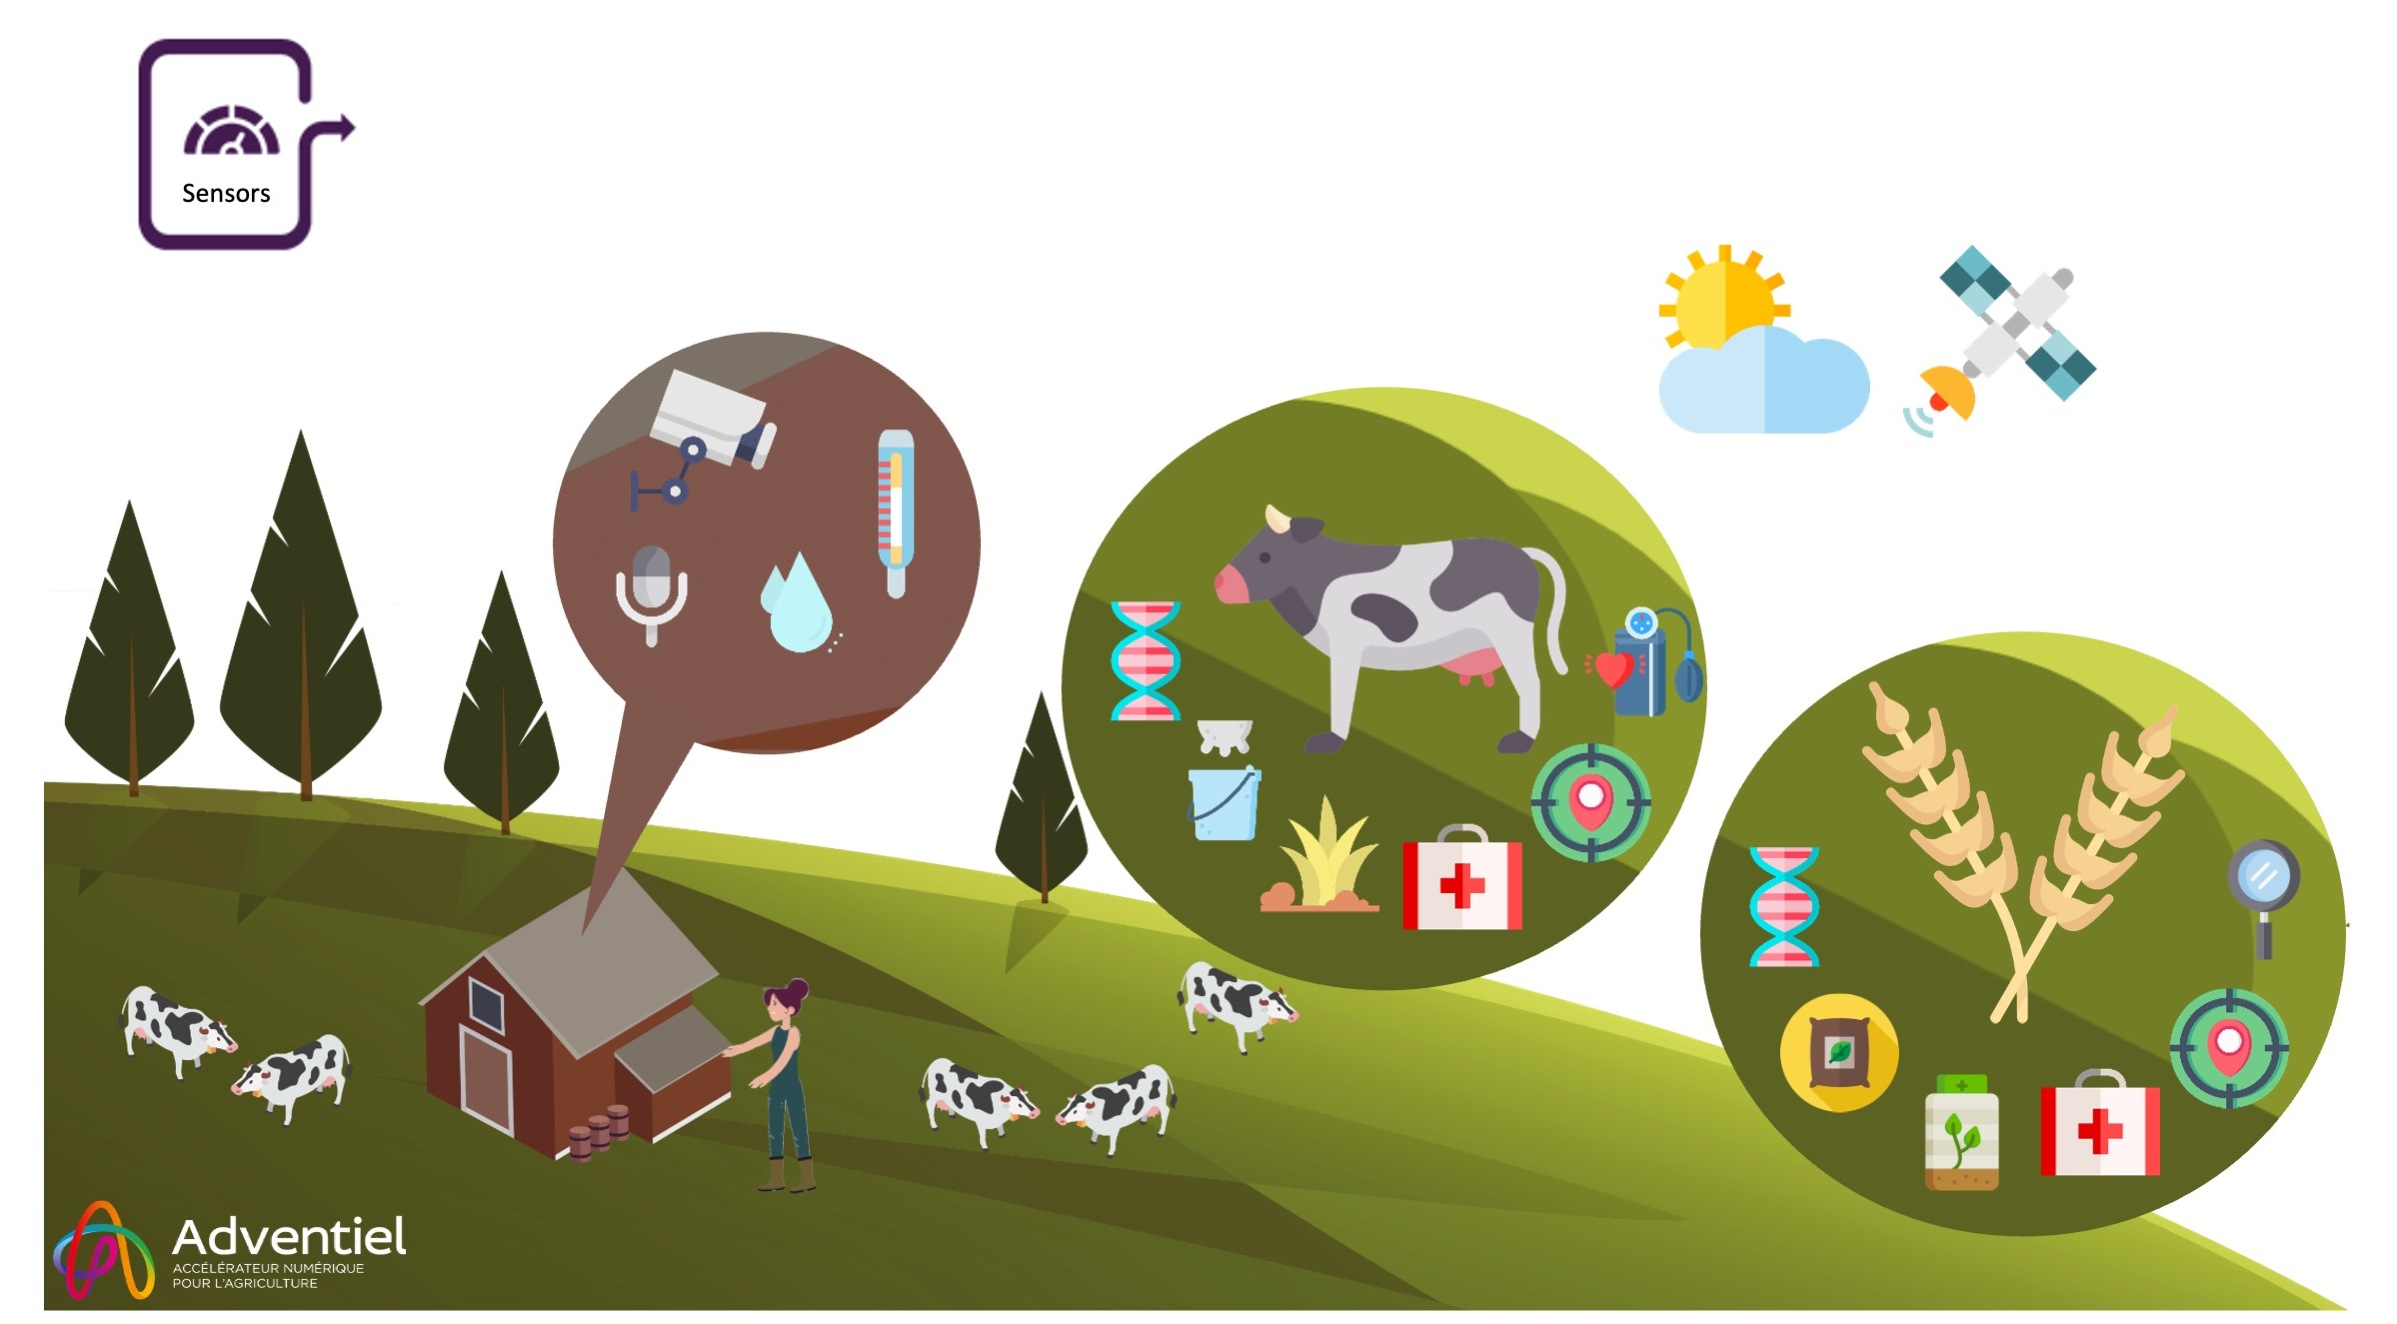
\includegraphics[width=\linewidth]{figures/chap1/chap1-sensors.jpg}
  \caption{Illustration of the diversere categories of observations that can be collected by sensor in livestock farming}
  \label{fig:chap1-sensors}
\end{figure}
\newpage

%%%%%%%%%

% Precision agriculture represents an innovative approach to farming that focuses on optimizing inputs (such as feed, medication, and energy) while maximizing outputs, including net profit and environmental sustainability. This paradigm is rapidly being adopted in livestock farming to enhance decision-making and operational efficiency. At its core, precision agriculture is supported by a robust infrastructure consisting of both hardware and software components. In this subsection, we concentrate on 



\subsection{Epidemiological modelling: Stochastic mechanistic models}

Mechanistic models in epidemiology have played a central role in translating complex, interdisciplinary insights into quantitative frameworks that inform evidence-based policy-making. Their construction begins by segmenting the population into compartments, typically susceptible, infected, and recovered, following seminal work by Bernoulli (1760), Ross (1916), and Kermack and McKendrick (1927) as detailed in early epidemiological studies. These foundational models not only formalized the understanding of disease transmission dynamics through systems of differential equations but also provided a platform for incorporating additional layers of biological, economic, and social theory into rule-based algorithms.

Building on these early models, researchers have developed increasingly sophisticated mechanistic models that integrate heterogeneous mixing patterns, demographic processes, and spatial structures. In the context of livestock infectious diseases, for instance, models have been extended to capture multi-scale interactions—from within-host processes to regional spread, thereby enabling the simulation of targeted interventions such as vaccination and movement restrictions 
\cite{Tomley2009, OIE2015}. The ability to embed theoretical insights into mathematical formulations allows these models to explore scenarios that are otherwise ethically or logistically infeasible to observe directly. This is crucial for policy-making, as it offers decision-makers evidence-based insights into the potential impacts of various control measures on both disease spread and animal welfare \cite{Ezanno2018, EZANNO2020100398}

The construction of these models generally involves formulating a set of differential equations or stochastic processes that describe transitions between defined compartments. Parameters such as the transmission rate, recovery rate, and contact structure are estimated using empirical data through methods like maximum likelihood estimation or Bayesian inference \cite{Keeling2008, Courcoul2010}. These fitting procedures are critical to ensure that the model outputs faithfully represent the underlying biological processes. However, a significant challenge arises from the increasing use of sensor-based data in modern epidemiological studies. Unstructured datasets, such as video and audio recordings from precision livestock farming, are rich in information yet notoriously difficult to process and integrate into these models due to the labour-intensive nature of manual data curation. The relevance of the model only depends on its use and the available data/knowledge to build and parametrize it. 

While preliminary efforts have begun to explore deep learning techniques for handling such unstructured data, the primary strength of mechanistic models lies in their capacity to consolidate interdisciplinary theoretical knowledge into a structured, predictive framework. This integration not only supports the evaluation of control strategies under diverse scenarios but also provides a safe, ethical alternative to field experimentation by simulating conditions that are hard to replicate in reality.


\subsection{Machine learning modelling: classical deep learning models}

Machine learning is an integral subfield of artificial intelligence that focuses on automatically deriving predictive models directly from datasets rather than embedding knowledge via mechanistic, rule‐based models such as those used in traditional epidemiology. In essence, it’s like teaching a child to recognize a cat by showing hundreds of pictures rather than providing explicit instructions \cite{rosenblatt1958perceptron}. At its core, deep learning creates multi-layered models that learn by adjusting their internal parameters based on examples. For instance, in image recognition, the first layers may detect simple features like edges and colours, while later layers combine these features to identify more complex patterns, such as the specific contours and textures that form a cat’s face \cite{Goodfellow-et-al-2016}. Early work in this area started with simple rule-based systems and perceptron models \cite{rosenblatt1958perceptron} and evolved over the decades into architectures that can span 10 to over 100 layers with tens to hundreds of millions of parameters \cite{Goodfellow-et-al-2016}. These deep models function as universal approximators, capable of modelling highly non-linear relationships by iteratively minimizing prediction error through back-propagation \cite{rumelhart1986learning} and stochastic gradient descent techniques that adjust millions of weights over thousands to millions of iterations using mini-batches of 32–512 samples \cite{hinton2012deep}. 

Among the classical deep learning models, several architectures have been particularly influential. Feed-forward neural networks serve as the basic building blocks in which data flows in one direction from input to output. Convolutional neural networks  have revolutionized computer vision by applying convolutional filters and max pooling operations to extract spatial hierarchies from high-resolution images (often 512×512 pixels or larger) and achieve translational invariance \cite{lecun1998gradient, krizhevsky2012imagenet}. Recurrent neural networks , and particularly their long short-term memory  variants, are engineered to handle sequential data by overcoming issues like the vanishing gradient problem through gating mechanisms, thus capturing dependencies that span thousands of time steps 
\cite{hochreiter1997long, graves2005framewise}. More recently, graph neural networks have emerged to model data with non-Euclidean structures—such as relationships in social networks or complex interactions on a farm \cite{scarselli2009graph}, while transformer models leverage self-attention mechanisms to process entire sequences in parallel, which improves the modelling of long-range dependencies and reduces training time \cite{vaswani2017attention}. In addition to these traditional architectures, foundational models—particularly large language models such as GPT (generative pre-trained transformer) have revolutionized natural language processing by being trained on vast amounts of text data to predict and generate human-like language \cite{brown2020language}. However, a significant challenge for these models is “hallucination,” where they generate plausible-sounding but factually incorrect or nonsensical outputs. This occurs because these models rely on statistical patterns rather than deep, mechanistic understanding, lacking strong theoretical grounding in the underlying principles of language \cite{marcus2020gpt3, bender2021stochastic}. In contexts like livestock management, where deep learning applications in natural language processing are used to analyse veterinary reports and sensor logs, such hallucinations can lead to false positive and incorrect diagnoses or misguided recommendations, highlighting the need for integrating explicit domain knowledge to improve reliability \cite{smith2020nlp}.

Because these deep learning models can have millions of parameters and many layers, they are often described as "black boxes" systems that deliver high accuracy yet offer little insight into how decisions are made. This opacity is problematic, especially in high-stakes domains such as healthcare, autonomous driving, or livestock management, where understanding a model’s rationale is crucial for safety and trust \cite{bengio2013representation}. Explainable Artificial Intelligence (XAI) addresses this gap by providing methods to interpret and understand the internal workings of complex models. For example, Gradient-weighted Class Activation Mapping (Grad-CAM) generates visual maps that indicate which parts of an image were most influential for the model’s decision, and Local Interpretable Model-agnostic Explanations (LIME) approximate a deep model’s local behaviour with a simpler, interpretable model for specific instances 
\cite{ribeiro2016should, selvaraju2017grad}. Another critical component is uncertainty quantification, which ensures that a model not only provides a prediction but also a measure of confidence in that prediction. Bayesian Neural Networks use variational methods to assign probability distributions to model parameters, so instead of providing a single fixed output, the network indicates, for example, that it is 90\% confident that an image contains a cat, with the remaining 10\% reflecting uncertainty \cite{gal_dropout_2016}. Similarly, conformal prediction techniques provide statistically valid prediction sets, ensuring that the true outcome is contained within these sets at a pre-defined confidence level \cite{Angelopoulos2021}.

Transformer-based models have been deployed to automatically analyse veterinary clinical records, social media posts from farmers, and sensor-generated text logs to identify early signs of disease outbreaks or stress in livestock populations \cite{smith2020nlp}. Deep learning models have also been used to monitor animal behaviour through video analysis, allowing for the  detection of anomalies such as lameness or aggressive behaviour, thereby enabling timely interventions that improve animal welfare and productivity 
\cite{fischer2018deep, kamphuis2017animal}. Other studies have demonstrated the utility of deep learning in livestock management by combining image analysis with sensor data. For example, CNNs have been used to automatically count and classify animals in large herds, while natural language processing helps in summarizing and integrating textual data from various reports, creating a comprehensive monitoring system that can alert farmers to potential issues before they escalate \cite{raboisson2017machine, bakker2019predictive, lopez2020integrated}.

All these techniques, deep neural architectures and its security techniques such as XAI methods and uncertainty quantification tools, come together to form a more robust and transparent system. By explaining their inner workings and providing confidence measures, these methods help users understand not only what the model’s decision is, but also why it made that decision and how reliable that decision is. This comprehensive approach is especially important in fields where decisions have significant consequences, such as in medical diagnosis, financial forecasting, or autonomous driving \cite{hinton2012deep, bengio2013representation}. Without integrating additional domain-specific knowledge, these models can struggle to generalize beyond the data on which they were trained, leaving significant opportunities for further research at the intersection of deep learning and mechanistic modelling. 


\subsection{Hybrid modelling: machine learning and epidemiological models}

Recent research in infectious disease modelling has sought to address the well‐known limitations of data‐driven and theoretical approaches when used in isolation. Deep learning methods, while highly effective at capturing complex, non-linear patterns from structured data, often struggle to extrapolate when confronted with untrained or sparse data. In contrast, mechanistic epidemiological models, which are built upon established theoretical principles of disease dynamics, frequently face challenges when fitting unstructured observations. This has led to the development of several hybrid integration approaches that aim to merge the complementary strengths of both methodologies to achieve objectives such as forecasting, model parametrization and calibration, intervention assessment and optimization, retrospective epidemic course analysis, transmission inference, and outbreak detection \cite{Ye2025}.

One prominent integration approach involves using Physics-Informed Neural Networks (PINNs) and Epidemiology-Augmented Artificial Models (EAAMs) to learn unknown components of epidemiological models. In these methods, deep learning architectures are augmented by incorporating epidemiological principles directly into the network—often through residual loss terms—to learn hidden state variables, parameters, or derivatives. This approach helps model parametrization and calibration while also improving forecasting capabilities by enforcing consistency with known epidemic dynamics. Studies employing this method have demonstrated its effectiveness on both real and synthetic datasets, as documented in recent literature \cite{kharazmi_identifiability_2021, barmparis_physicsinformed_2022, de_rosa_modelling_2023, torku_seinn_2023,berkhahn_physics-informed_2022, rodriguez_einns_2023, shaier_data-driven_2022, bertaglia_asymptotic-preserving_2022, malinzi_determining_2022} for PINNs; \cite{liu_rolling_2023, otadi_universal_2017, liu_epidemiology-aware_2023, amini_mepognn_2023, sun_2022, gao_stan_2021, zheng_spatial-temporal_2021, ma_enhancing_2022, wang_causalgnn_2022, nguyen_becaked_2022, nguyen_becaked_2022-1} for EAAMs 

% and \cite{wang_tdefsi_2020, zhan_optimizing_2021, wang_deep_2021, bogacsovics_replacing_2021, wang_predicting_2022, murphy_deep_2021, zhang_understanding_2021, quilodran-casas_digital_2022, silva_data_2022}
%[69–77, 78–88].

Another strategy leverages mechanistic models to generate synthetic datasets under varied parameter conditions. Deep learning architectures, such as recurrent neural networks, are then trained on these synthetic datasets to predict unobserved model components or forecast future epidemic trajectories. By doing so, this approach addresses the challenge of limited real-world data and contributes significantly to both forecasting and transmission inference. The synthetic data enable the model to generalize beyond the training domain, thereby enhancing its capacity to infer underlying transmission patterns in scenarios where observational data are sparse \cite{petrica_inverse_2023,liu_prediction_2023,rahnsch_network-based_2024,kumar_epidemic_2023,ji_climate-dependent_2023,vega_simlr_2022,chen_covid-19_2023,alsmadi_susceptible_2023,qiu_prediction_2022,mu_modelling_2023,wang_machine_2021,wu_computer_2022,yao_assessment_2022,zhang_prediction_2021,wyss_modeling_2023,gadewadikar_methodology_2024,zisad_integrated_2021,merkelbach_hybridml_2022,munoz_hybrid_2022,castillo_ossa_hybrid_2021,jiang_countrywide_2021,yasami_application_2022,liao_sirvd-dl_2021,zheng_predicting_2020,watson_pandemic_2021,liu_nesting_2023,wang_policy_2022,wang_hypothesis-free_2022,deng_dynamics_2020,kim_determination_2021,gupta_deep-siqrv_2023,bousquet_deep_2022,feng_data_2022,ding_biology-informed_2023,khan_attention_2022,kumaresan_analysis_2022,long_identification_2021}

A further integration approach embeds epidemiological constraints directly within deep learning frameworks. By incorporating established conservation laws or differential equations into the model’s inputs, loss functions, or architecture, these hybrid models ensure that predictions adhere to the theoretical underpinnings of disease dynamics. This method improves both the accuracy of forecasts and the robustness of retrospective epidemic course analyses by aligning data-driven predictions with fundamental epidemiological knowledge \cite{kharazmi_identifiability_2021,barmparis_physicsinformed_2022,de_rosa_modelling_2023,torku_seinn_2023,berkhahn_physics-informed_2022,rodriguez_einns_2023,shaier_data-driven_2022,bertaglia_asymptotic-preserving_2022,malinzi_determining_2022}. In a related vein, reinforcement learning and optimal control frameworks have been integrated into simulation environments derived from mechanistic models. In these approaches, reinforcement learning agents interact with epidemiologically informed simulations to iteratively optimize intervention strategies. This methodology directly addresses the objective of disease intervention assessment and optimization by enabling the exploration of optimal control policies through continuous feedback from the simulation environment \cite{yao_optimal_2023,zou_data-efficient_2021,vereshchaka_optimization_2021,song_reinforced_2020,probert_context_2019,ohi_exploring_2020,khadilkar_optimising_2020,hao_reinforcement_2022,libin_deep_2021,awasthi_vacsim_2022,song_robust_2023,padmanabhan_reinforcement_2021,kompella_reinforcement_2020,mai_planning_2023,asikis_neural_2022,roy_knowledge_2021,colas_epidemioptim_2021,capobianco_agent-based_2021,ou_active_2021,trad_towards_2022,bushaj_simulation-deep_2022,chadi_2022 ,guo_pacar_2022,kulkarni_optimizing_2022,deng_optimal_2021,hwang_optimal_2022,wan_multi-objective_2022,miralles-pechuan_methodology_2020,bampa_epidrlearn_2022,shami_economic_2022,du_district-coupled_2022,benalcazar_deep_2021,xia_controlling_2022,khatami_reinforcement_2021,zong_reinforcement_2022,du_hrl4ec_2023,nguyen_general_2022,beigi_application_2021} for RL methods and \cite{yin_optimal_2023,asikis_neural_2022,courtes_reduced_2024,li_robust_2021,kmet_neural_2023,kmet_bezier_2019} for optimal control frameworks.

Additional integration strategies focus on enhancing the quality of unstructured observational data and reducing prediction error. Techniques such as support vector machines and tree-based classifiers are applied to extract auxiliary information from heterogeneous datasets, thereby refining parameter estimation and indirectly supporting retrospective analysis and outbreak detection. Moreover, ensemble modelling methods, which combine outputs from independently trained models through stacking, boosting, or bagging, have been shown to reduce overall prediction error and increase robustness. These ensemble techniques facilitate improved forecasting accuracy and more reliable outbreak detection by synthesizing diverse model predictions \cite{tuarob_modeling_2015,solares-hernandez_adaptation_2023,rosato_extracting_2023,kandula_improved_2019} and 
\cite{kandula_evaluation_2018,adiga_all_2021,nadler_neural_2020,maniamfu_lstm-based_2023,adiga_enhancing_2022,delli_compagni_hybrid_2022}. Complementing these methods, Bayesian neural networks have been employed to quantify uncertainty in parameter inference. By approximating the posterior distribution of model parameters, this approach provides critical measures of confidence that enhance forecasting, transmission inference, and outbreak detection \cite{ryder2018blackboxvariationalinferencestochastic, ARNST2022108805, 10.1371/journal.pcbi.1005416, 10.1371/journal.pcbi.1009472}. Finally, clustering-based decomposition uses unsupervised learning algorithms, such as k-means, to partition large-scale epidemiological models into smaller sub-models. This segmentation enables localized analysis and tailored intervention strategies, thereby strengthening retrospective epidemic course analysis and improving the sensitivity of outbreak detection \cite{bertozzi-villa_archetypes_2023}.

Among the studies reviewed, a total of 26 infectious diseases were investigated using integrated models. Notably, COVID-19 dominated the research landscape, accounting for 60\% of the studies, with 148 investigations dedicated to this disease. Influenza was the focus in 7\% of the studies, dengue in 2\%, and HIV in 1\%. In addition, 23\% of the studies utilised hypothetical disease scenarios to demonstrate the applicability of the methods. Based on the reviewed studies, there isn’t strong evidence that sensor observations—such as data directly collected from IoT devices or on‐farm sensors—have been prominently integrated into these frameworks. Some work has explored the use of sensor‐based data like satellite imagery (which is one form of sensor observation) to capture environmental factors. However, most approaches in the review primarily rely on traditional surveillance data and non‑traditional sources such as social media, search queries, or emergency reports, rather than sensor observations from livestock or similar settings. This represents an opportunity for future research to incorporate direct sensor data for automated monitoring and relevant context-specific insights.


%%%%%%%%%
% This section serves as a concise narrative review of various methodologies for integrating machine learning models with epidemiological models, offering a critical perspective on their limitations. Addressing these limitations is central to the contributions of this thesis.

% This section presumes that the reader possesses a foundational understanding of ensemble techniques in modelling, specifically bagging, boosting, and stacking. They are pivotal in enhancing the global performance by combining multiple models. These methods aim to reduce errors, improve accuracy, and increase the robustness of predictions. Stacking Combines outputs from several distinct models using an additional "meta-model," learning optimal combinations for improved predictions. Boosting refers to sequentially training multiple weak predictive models, each aiming to correct errors from previous models, thus progressively improving overall prediction accuracy. Bagging (or Bootstrap Aggregating) refers to parallel training of multiple unique models (while stacking used distinct models, bagging uses multiple instances but of the same model) on random subsets of data (with replacement), thereby reducing prediction variance and mitigating over-fitting.



% En sciences, toute tentative de tirer des conclusions généralisables nécessite un
% modèle, i.e. une version abstraite de la réalité \cite{McCallum2008}. Cette représentation
% abstraite est dotée d’un objectif (a model is a "purposeful representation", 
% \cite{Starfield1990}, qui requiert un certain degré de simplification.




% Methodologicaly-wise, these models can also grouped into nine primary integration approach. Figure \ref{fig:chap1-hybrid} illustrates several methodological frameworks that integrate machine learning with mechanistic epidemiological models.  In the first integration method—Learning Unknown Components of Epidemiological Models, AI models (namely PINNs, EAAMs, and synthetically-trained AI models) are employed to “learn” the unknown elements of mechanistic models, such as state variables, parameters, or derivatives. The integration is achieved by incorporating epidemiological principles,often in the form of residual loss terms—directly into the network architecture, as shown in figure \ref{fig:chap1-hybrid} (subplot c) The training process consists of end-to-end supervised training using gradient-based optimization (e.g., Adam or SGD) applied on real or synthetic datasets. The original citations for this method are \cite{kharazmi_identifiability_2021, barmparis_physicsinformed_2022, de_rosa_modelling_2023, torku_seinn_2023,berkhahn_physics-informed_2022, rodriguez_einns_2023, shaier_data-driven_2022, bertaglia_asymptotic-preserving_2022, malinzi_determining_2022} for PINNs; \cite{liu_rolling_2023, otadi_universal_2017, liu_epidemiology-aware_2023, amini_mepognn_2023, sun_2022, gao_stan_2021, zheng_spatial-temporal_2021, ma_enhancing_2022, wang_causalgnn_2022, nguyen_becaked_2022, nguyen_becaked_2022-1} for EAAMs; and \cite{wang_tdefsi_2020, zhan_optimizing_2021, wang_deep_2021, bogacsovics_replacing_2021, wang_predicting_2022, murphy_deep_2021, zhang_understanding_2021, quilodran-casas_digital_2022, silva_data_2022}.

% The second method—Training AI Models Using Synthetic Data (Fig \ref{fig:chap1-hybrid} subplot e), uses mechanistic models to generate synthetic datasets under varying parameter conditions. In this approach, AI models such as recurrent neural networks (RNNs) are trained on these synthetic datasets with the aim of predicting unknown model components or future epidemic trajectories. The training is performed using standard supervised learning methods on synthetic data. The corresponding citations for this method are \cite{petrica_inverse_2023,liu_prediction_2023,rahnsch_network-based_2024,kumar_epidemic_2023,ji_climate-dependent_2023,vega_simlr_2022,chen_covid-19_2023,alsmadi_susceptible_2023,qiu_prediction_2022,mu_modelling_2023,wang_machine_2021,wu_computer_2022,yao_assessment_2022,zhang_prediction_2021,wyss_modeling_2023,gadewadikar_methodology_2024,zisad_integrated_2021,merkelbach_hybridml_2022,munoz_hybrid_2022,castillo_ossa_hybrid_2021,jiang_countrywide_2021,yasami_application_2022,liao_sirvd-dl_2021,zheng_predicting_2020,watson_pandemic_2021,liu_nesting_2023,wang_policy_2022,wang_hypothesis-free_2022,deng_dynamics_2020,kim_determination_2021,gupta_deep-siqrv_2023,bousquet_deep_2022,feng_data_2022,ding_biology-informed_2023,khan_attention_2022,kumaresan_analysis_2022,long_identification_2021} .

% Another approach embeds epidemiological knowledge directly into AI models. In this method, known epidemiological constraints, such as conservation laws or differential equations that govern disease spread—are integrated into the AI model’s inputs, loss functions, or architecture. The objective is to enforce that the predictions adhere to established epidemic dynamics. This method typically uses gradient-based supervised training on real datasets, although synthetic data may also be incorporated. (Fig \ref{fig:chap1-hybrid} subplot a \& d) outlines the architecture where epidemiological inputs and custom loss functions work together to constrain the learning process. The studies related to this method are detailed in the related references \cite{kharazmi_identifiability_2021,barmparis_physicsinformed_2022,de_rosa_modelling_2023,torku_seinn_2023,berkhahn_physics-informed_2022,rodriguez_einns_2023,shaier_data-driven_2022,bertaglia_asymptotic-preserving_2022,malinzi_determining_2022}.

% The next method focuses on optimal decision-making through AI models, particularly using reinforcement learning (RL) or optimal control frameworks. In these approaches, mechanistic models provide simulated environments where RL agents learn optimal intervention strategies through iterative interactions. The training process involves training RL agents within epidemiologically based environments or using neural networks to approximate control variables through iterative optimization techniques. The method has been applied to assess intervention policies in settings like the COVID-19 pandemic. (Fig \ref{fig:chap1-hybrid} subplot h) displays the interaction between the RL agent and the simulation environment, highlighting the iterative nature of the learning process. The original citations for this method are \cite{yao_optimal_2023,zou_data-efficient_2021,vereshchaka_optimization_2021,song_reinforced_2020,probert_context_2019,ohi_exploring_2020,khadilkar_optimising_2020,hao_reinforcement_2022,libin_deep_2021,awasthi_vacsim_2022,song_robust_2023,padmanabhan_reinforcement_2021,kompella_reinforcement_2020,mai_planning_2023,asikis_neural_2022,roy_knowledge_2021,colas_epidemioptim_2021,capobianco_agent-based_2021,ou_active_2021,trad_towards_2022,bushaj_simulation-deep_2022,chadi_2022 ,guo_pacar_2022,kulkarni_optimizing_2022,deng_optimal_2021,hwang_optimal_2022,wan_multi-objective_2022,miralles-pechuan_methodology_2020,bampa_epidrlearn_2022,shami_economic_2022,du_district-coupled_2022,benalcazar_deep_2021,xia_controlling_2022,khatami_reinforcement_2021,zong_reinforcement_2022,du_hrl4ec_2023,nguyen_general_2022,beigi_application_2021} for RL methods and \cite{yin_optimal_2023,asikis_neural_2022,courtes_reduced_2024,li_robust_2021,kmet_neural_2023,kmet_bezier_2019} for optimal control frameworks.

% Enhancing observational data constitutes another integration strategy. Here, AI techniques—using methods such as support vector machines or tree-based classifiers, are employed to extract auxiliary information (infer health status and generate enhanced observational datasets) from non-traditional data sources (e.g., text from social media, emergency reports) and improve the quality of conventional epidemiological datasets. This method, which generally relies on real data, refines model parameter estimation. (Fig \ref{fig:chap1-hybrid} subplot b) illustrates how enhanced data inputs feed into the epidemiological model to improve its performance. The original citations for this method are \cite{tuarob_modeling_2015,solares-hernandez_adaptation_2023,rosato_extracting_2023,kandula_improved_2019}.

% Ensemble modelling of AI and epidemiological models is yet another integration approach where outputs from distinct models are combined using techniques like weighted averaging, stacking, or boosting, to improve forecasting accuracy.  In this framework, individual models are first trained separately on either real or synthetic data; subsequently, a meta-model (for instance, an LSTM-based stacker) is trained on historical performance to combine these outputs into a final forecast. The original citations for this approach are \cite{kandula_evaluation_2018,adiga_all_2021,nadler_neural_2020,maniamfu_lstm-based_2023,adiga_enhancing_2022,delli_compagni_hybrid_2022}. This approach has been applied, for instance, in COVID-19 forecasting, and (Fig \ref{fig:chap1-hybrid} subplot f)depicts the ensemble process with multiple model outputs converging into a final prediction.

% One approach employs Bayesian neural networks to enhance parameter inference within mechanistic epidemiological models. In this framework, the neural network is structured to quantify uncertainty by approximating the posterior distribution of model parameters, a critical capability when dealing with intractable likelihoods or limited data. The training process typically involves optimizing variational objectives, such as maximizing the evidence lower bound (ELBO), using real-world observational datasets. (Fig \ref{fig:chap1-hybrid} subplot g) illustrates the architecture that integrates uncertainty quantification directly into the model. The original studies detailing this approach are referenced in \cite{ryder2018blackboxvariationalinferencestochastic, ARNST2022108805, 10.1371/journal.pcbi.1005416, 10.1371/journal.pcbi.1009472}.

% Lastly, clustering-based decomposition of epidemiological models (Fig \ref{fig:chap1-hybrid} subplot i) offers a means to break down large-scale, complex models into smaller, more manageable sub-models. By applying clustering algorithms (such as k-means) to group regions or populations with similar epidemic characteristics, this approach allows for localized analysis and tailored intervention strategies. Typically leveraging unsupervised learning, these methods primarily work with real-world data but can also incorporate synthetic data in simulation studies. They are particularly useful for targeted outbreak detection and evaluation of region-specific intervention impacts \cite{bertozzi-villa_archetypes_2023} . Figure 1.1 provides a schematic of how clustering methods break down the overall model into manageable sub-models.

% \begin{itemize}
%     \item Physics-Informed Neural Networks (PINNs): PINNs integrate known governing equations (e.g., differential equations describing infectious dynamics) as soft constraints into neural networks during training. The neural network is guided by both observed data and theoretical knowledge, ensuring physically plausible predictions and improved extrapolation beyond the training distribution.
%     \item Neural Differential Equations (Neural ODEs/SDEs): Neural ODEs or SDEs embed neural networks into differential equations, allowing the modelling of dynamic processes through continuous-time representations. Such integration directly captures temporal dynamics, offering more flexibility and interpretability compared to classical discrete-time deep learning methods.
% \end{itemize}

% Despite their promising advantages, hybrid and ensemble models have inherent challenges:
% Despite notable advancement in the scientific community, there is a conceptual gap, between the raw unstructured livestock data that can be captured and the strong theoretical knowledge we have of the complex underlying infectious mechanisms. This basically allows to ground the theoretical knowledge we have on a complex mechanisms to the context-specific observations, hence harness the best of both world. 

% \begin{figure}[h]
%   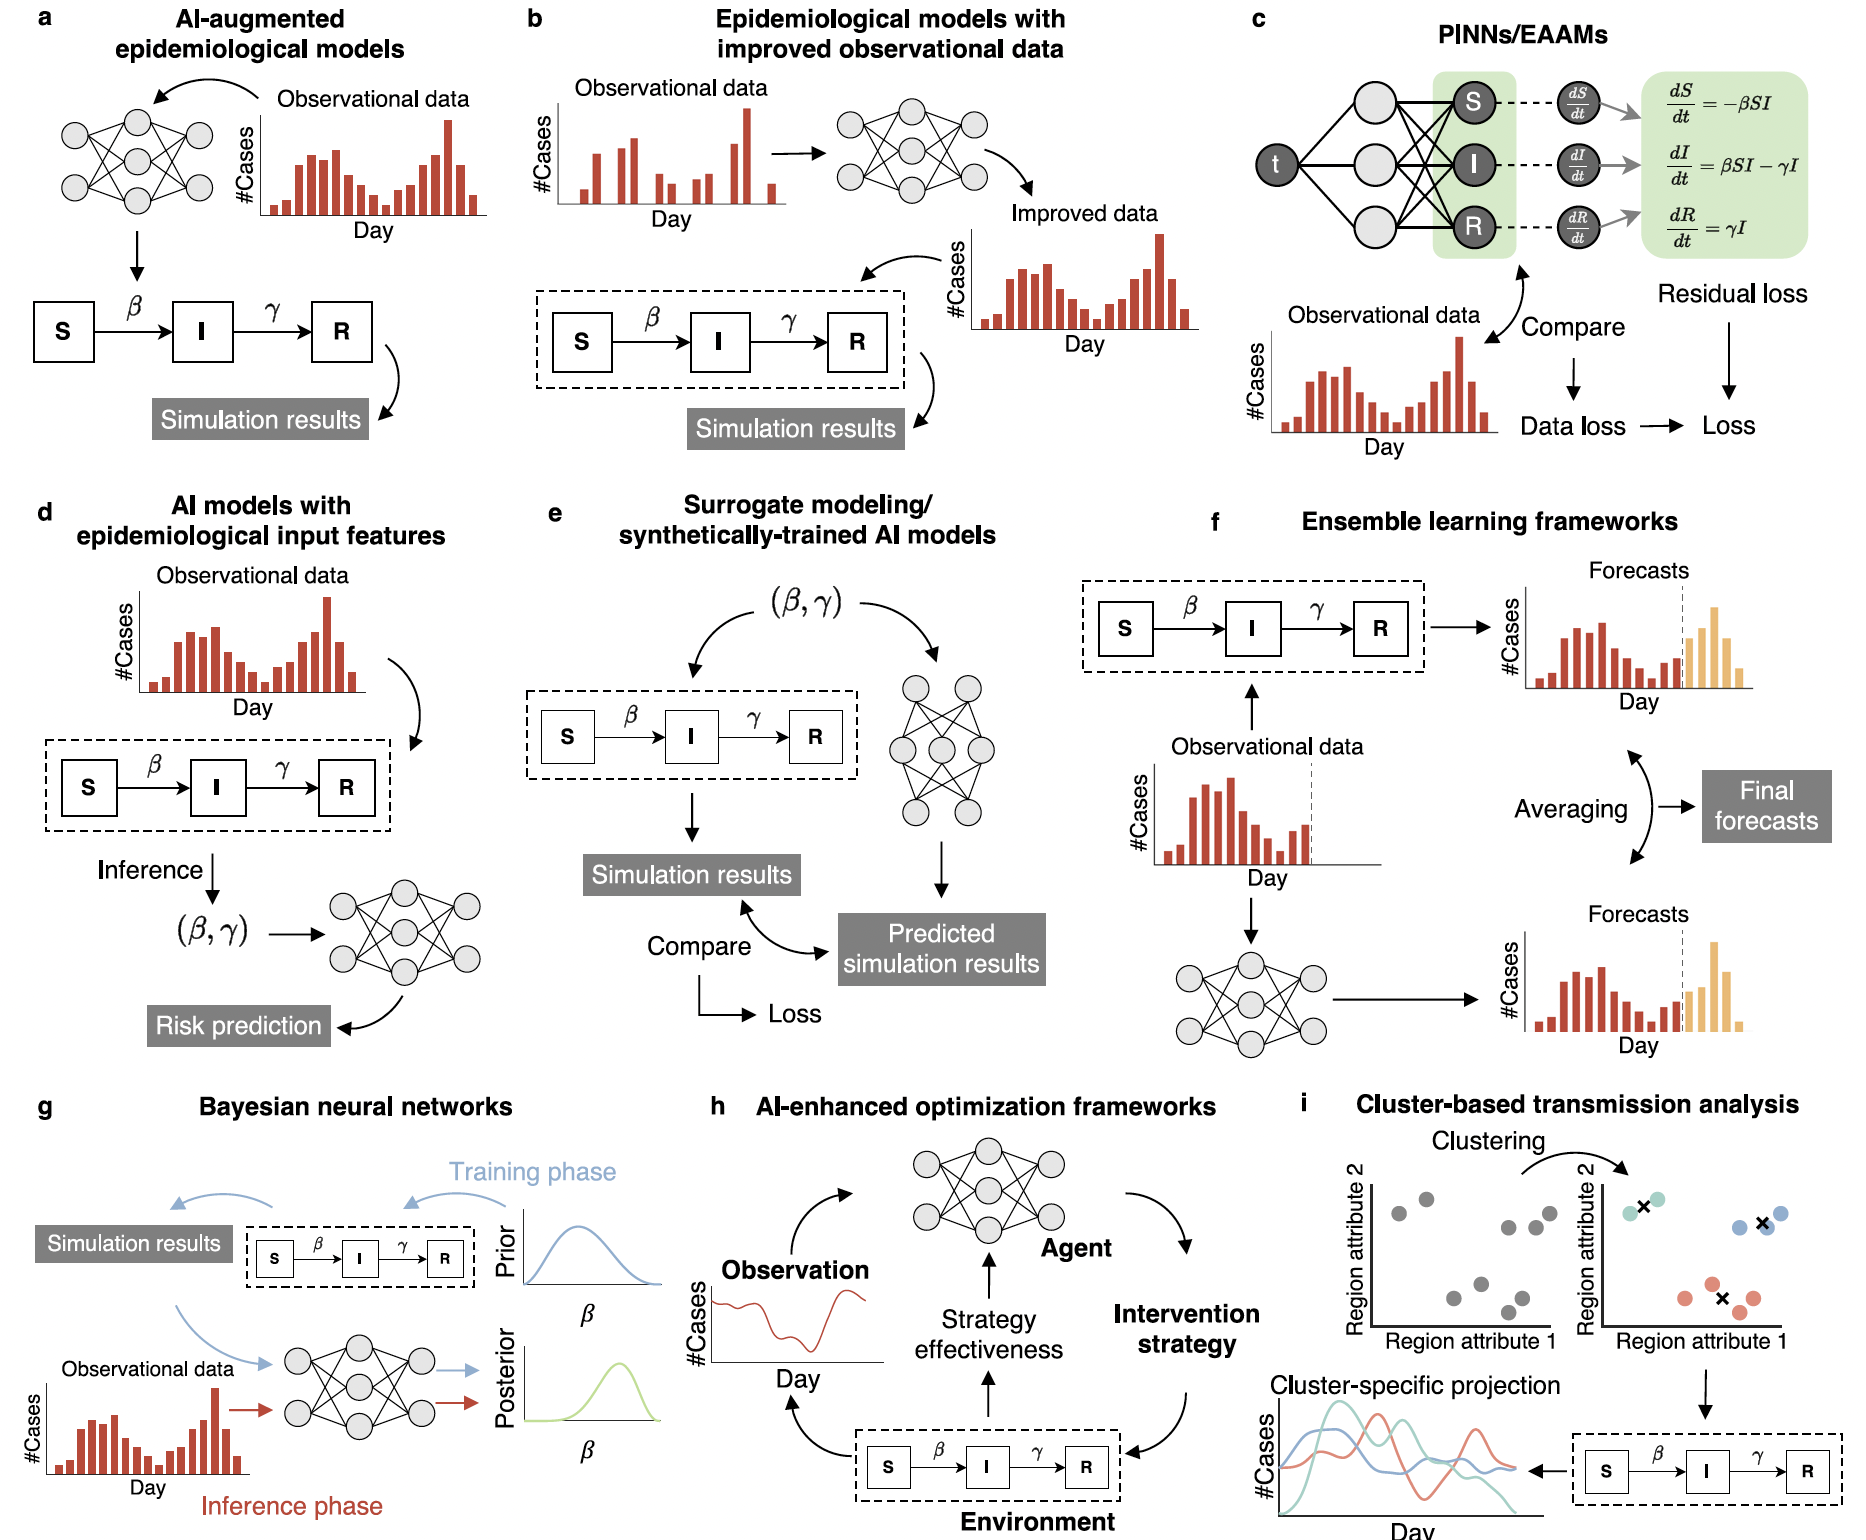
\includegraphics[width=\linewidth]{figures/chap1/chap1-hybrid.png}
%   \caption{Illustrative examples of methodological frameworks coupling Machine learning and epidemiological models}
%   \label{fig:chap1-hybrid}
% \end{figure}


% Among the studies reviewed, a total of 26 infectious diseases were investigated using integrated models. Notably, COVID-19 dominated the research landscape, accounting for 60\% of the studies, with 148 investigations dedicated to this disease. Influenza was the focus in 7\% of the studies, dengue in 2\%, and HIV in 1\%. In addition, 23\% of the studies utilized hypothetical disease scenarios to demonstrate the applicability of the methods, rather than concentrating on a specific infectious disease. These are studies that are the closest to the question this thesis is trying to bring a part of answer to.


% Each ensemble strategy presents specific strengths and limitations, related to computational complexity, interpretability, and predictive power. 
% research gaps:
% \begin{itemize}
%     \item Generalizability: The majority of integrated models focus on diseases like COVID-19, limiting applicability to other infectious diseases with indirect or complex transmission routes.
%     \item Expansion beyond COVID-19 to other diseases with indirect transmission mechanisms.
%     \item Data Limitations: Many studies depend on synthetic or limited real-world data, highlighting the need for richer, real-time data integration (e.g., satellite imagery, social media data). - we have gathered in this thesis a real-wolrd multi-modal dataset (...)
% \end{itemize}

% je vais enlever cette subsub section, elle ne sert à rien
% \subsubsection*{Maintainability}

%     \begin{itemize}
%         \item strongly coupled methods requires the builder to be deeply understand the problematic of domain in order to implement the models. (full stack vs frontend or backend). So retraining for example would require the whole system to be trained and in the long-term, it would also require sort of full-stack builders. 
        
%         \item strongly coupled methods would still require a  certain quantity of data since in order for example for the deep learning model to fine-tune the mechanistic model (neural differential equations). Usually ensembled model (so more parameters) would require more dimensions in order to fit all the parameters (curse of dimensionality)
%     \end{itemize}

% le domaine est très large, mais nous on va se focaliser uniquement sur le couplage deep et modèle méchaniste de façon générale. 

% sachant que nous c'est une forme de boosting, sans trop de redondances,) et surtout découplé (faiblement couplé) - ceci sont des couplages forts mais comme un site web à egalement ces limites. comme un développeur full stack - parler rapidement des NDE, des pinns qui sont juste une sous familles des NDE.



%----------------------------------------------------------------------------------------
%	SECTION 
%----------------------------------------------------------------------------------------
\clearpage 

\section{Thesis objective and outline}

\subsection{Exploring the complementarities between deep learning and mechanistic epidemiological models}

Precision agriculture provides powerful tools enabling automation of real-world observations through various sensors. Throughout this thesis, we have leveraged such tools to acquire contextual observational data essential for studying an infectious disease in livestock farming. However, sensor-based observations, although rich and increasingly accessible, represent only partial information regarding complex and unpredictable disease dynamics, aptly summarized by Yoan Bourhis (2017): "Nos observations ne révèlent que la partie émergée d’un iceberg au comportement complexe et peu prévisible."

Thus, a central question guiding this thesis is: How can sensor observations be effectively employed to study infectious diseases and support informed decision-making?

Our main hypothesis is that the most scientifically robust approach to contemporary quantitative questions in animal health, particularly regarding livestock infectious diseases, lies in combining complementary artificial intelligence methods, specifically deep learning and mechanistic epidemiological models. Such integration leverages deep learning’s capabilities for processing and extracting short-term insights from unstructured (video, image or text) observations  and the extrapolative capacities of stochastic epidemiological models grounded in explicit theoretical knowledge for long-term insights. This combination aims to better link real-world observations obtained through sensors with our theoretical knowledge in order make make relevant evidence-based recommendations at a larger temporal scales.

This naturally raises another foundational question addressed in this thesis:
In what ways can deep learning complement mechanistic epidemiological models in epidemiology ?

Complex animal health problems, including the study and control of infectious diseases, require distinct yet interconnected types of expertise: diagnosing diseases from immediate observational data, making reliable prognoses about future disease dynamics, and ultimately providing actionable recommendations. Diagnosis relies predominantly on processing unstructured field observations from sensors—thus favouring deep learning. Robust prognosis, however, relies on explicit theoretical knowledge and interpretability—domains inherently suited to mechanistic models. Finally, the quality of actionable recommendations is critically dependent on effectively bridging these two forms of expertise.

This thesis proposes a loosely coupled methodology inspired by the statistical principle known as the "Mixture of Experts" (MoE). This modular integration allows each expert to specialize explicitly in its distinct role (diagnosis and prognosis), enhancing accuracy, resource efficiency, interpretability, and scalability.

Addressing these considerations, the scientific questions explored throughout this thesis are:

\begin{enumerate}
    \item To what extent can deep learning reliably automate short-term diagnosis using limited, noisy, and context-specific observational data from sensors, such as lung ultrasounds ? 
    
    \item How can mechanistic epidemiological models be reliably parametrized using empirical veterinary observations to provide accurate long-term prognosis for infectious diseases ?
    
    % \item Given multiple mechanistic epidemiological models validly representing different expertise symptomatic dynamics of infectious diseases, how can observational data alone reliably guide the selection of the most appropriate mechanistic model to enable pathogen-specific disease management ?
    
    % \item How can observational data alone guide the selection of the best mechanistic prognosis expert when they are multiple epidemiological models expert for expliciting different mechanisms of the infectious disease.
    
    \item Given multiple mechanistic epidemiological models representing different but valid expertise in prognosing an outbreak, how can observational data alone reliably guide the selection of the most appropriate mechanistic model to enable pathogen-specific disease management.

    \item How can deep learning and mechanistic models be effectively integrated into a hybrid diagnostic-to-prognostic pipeline that leverages their complementary strengths to improve livestock disease management ?
    
    \item How can uncertainties inherent in sensor-based observations be explicitly accounted for within a hybrid modelling approach, and how does this influence diagnostic and prognostic reliability ?
\end{enumerate}


\textit{\textbf{Keywords:}} methodological synergy, complementary expertise, deep learning, mechanistic epidemiological models, diagnostic accuracy, prognostic reliability, uncertainty quantification, Mixture of Experts, modular architecture, scalability.

\subsection{Application to study Bovine Respiratory Diseases}
% In this subsection, I want to show that BRD are a good example for the application of our methodology

Bovine Respiratory Diseases (BRD) refer to a group of complex, multifactorial infectious disorders predominantly affecting young cattle in fattening farms. They are characterized by inflammation of the respiratory tract, causing symptoms such as cough, nasal discharge, fever, reduced feed intake, impaired growth, and occasionally, death. Although several pathogens (viruses, bacteria, mycoplasma) contribute to BRD, their clinical presentation is frequently non-specific, complicating accurate and timely diagnosis.

Diagnosing and managing BRD effectively remains notoriously challenging for several reasons:
\begin{itemize}
    \item Non-specific Clinical Signs: Clinical manifestations of BRD (e.g., cough, fever) are highly unspecific and overlap significantly with other diseases. Consequently, visual appraisal by farmers and veterinarians often results in misdiagnoses or delayed diagnoses, leading to suboptimal treatment strategies.
    \item Limitations of Biological Diagnostic Methods: Laboratory methods (e.g., Polymerase Chain Reaction (PCR), serology) provide increased specificity and accuracy compared to clinical appraisal alone. However, these tests are invasive, expensive, and time-consuming, delaying actionable results and increasing animal stress and discomfort. Moreover, logistical issues frequently limit their practicality, especially in large-scale operations.
    \item False Positives and Diagnostic Uncertainty: Due to the multifactorial nature of BRD (co-infections, pathogen interactions, host susceptibility variability), diagnostic and prognostic accuracy remain challenging. These difficulties result in inappropriate usage of antimicrobials, contributing to the rising threat of antimicrobial resistance and negatively impacting animal welfare.
\end{itemize}

(Complexity of BRD Etiology) BRD arises from complex interactions between intrinsic and extrinsic factors:
\begin{itemize}
    \item Pathogen Diversity and Interactions: Multiple pathogens (e.g., Mannheimia haemolytica, Pasteurella multocida, Bovine Respiratory Syncytial Virus, etc.) are frequently involved, potentially interacting in complex and poorly understood ways. Current veterinary research continues to explore these interactions to better characterize clinical markers useful for early detection, prognosis, and improved control measures (as exemplified in recent doctoral works, e.g., Maud’s research).
    \item Influence of Environmental and Management Practices: External factors such as farm management, biosecurity measures, herd density, transportation stress, and climatic conditions profoundly influence the occurrence and severity of BRD outbreaks. This intrinsic and extrinsic complexity significantly complicates disease modelling, prognosis, and control efforts.
\end{itemize}


(Socioeconomic Impact of BRD in Livestock Farming) Bovine Respiratory Diseases represent a major health and economic burden for farmers, veterinarians, and the broader livestock industry:
\begin{itemize}
    \item Economic Costs and Mortality Rates: BRD accounts for substantial economic losses in terms of reduced growth performance, increased mortality rates, and heightened veterinary and medicinal expenses. Particularly in French beef fattening farms, BRD is considered one of the most prevalent and economically significant animal health problems.
    \item Antimicrobial Usage and Ethical Concerns: Frequent misdiagnosis or delayed interventions lead to inappropriate use of antibiotics, fostering antimicrobial resistance. This concern raises ethical, public health, and animal welfare issues and highlights the urgent need for improved diagnostics and targeted therapeutic approaches.
\end{itemize}

(Existing Technological Approaches and Limitations) Recent research has applied sensor technologies (e.g., intra-ruminal temperature sensors, accelerometers, audio and video analytics) coupled with traditional machine learning and deep learning methods to improve BRD detection. Although promising, these data-driven approaches often:
\begin{itemize}
    \item Exhibit high false-positive rates due to limited specificity in clinical signs or ambiguous sensor outputs.
    \item Require substantial volumes of training data to achieve reliable performance, a constraint given practical difficulties in generating extensive labelled datasets.
    \item Struggle to predict disease progression or forecast epidemiological outcomes accurately over extended periods, thus limiting their use in proactive disease management and intervention strategies.
    \item Lack the capability to explore unobservable scenarios, such as hypothetical outbreaks or unrecorded infections, limiting their utility for scenario-based disease control planning.
\end{itemize}

There are also been mechanistic models developed before and throughout this thesis to model and study BRD (see Originality of this thesis). They have never applied to real-world observations. In this thesis, we employed these models to assess our methodology.

By bridging sophisticated deep learning feature extraction with robust, interpretable mechanistic models, this hybrid approach could significantly advance the ability to manage BRD effectively—improving animal health, welfare, farm economics, and sustainability and ecological issues. 

This thesis leverages BRD as a scientifically significant case study to validate a hybrid deep-mechanistic methodology, explicitly addressing the limitations noted above, with the aim of substantially improving diagnosis, prognosis, and disease management strategies in livestock farming.

\textit{\textbf{Keywords:}} Bovine Respiratory Disease, infectious disease dynamics, antimicrobial resistance, multi-modal data integration, predictive analytics, animal welfare.


\subsection{Originality of this thesis}


\paragraph{interdisciplinarity: synergy of diverse domain expertise }
% In this subsection, I want to explain the thesis CIFRE, with the mixture of domain expertise: epidemiological mechanistic modelling, statistical inference approaches, computer vision and deep learning, hardware and software engineering Mais également la collaboration avec les vétos. Préciser que c'est une thèse cifre (ce que peut apporter/ et les gains en retours pour adventiel: les côté applicatif, igepp (deep), Dynamo (mécaniste, inférence...). It is original to have as many different domain experts come together to work on one subject right ?

Uniquely structured via a CIFRE agreement, this thesis integrates expertise from diverse domains:  
\begin{itemize}
    \item Adventiel: Providing strong expertise in software and hardware engineering for precision agriculture, particularly focusing on practical applications, technical robustness, and user-friendly decision support tools.
    \item BIOEPAR-dynamo: Offering significant theoretical and applied expertise in mechanistic epidemiological modelling and statistical inference methods, including parameter inference and calibration techniques, tailored specifically to livestock disease dynamics. Emulsion (generic simulation engine for epidemiological mechanistic models)
    \item IGEPP-demecologie: Contributing substantial expertise in statistical inference, deep learning, and computer vision methodologies.
    \item Collaborations established through multi-partner projects such as SEPTIME and MULTIPAST, involving key contributors (e.g., Baptiste-Sorin), enhance the thesis’s capacity to integrate different forms of scientific expertise.
\end{itemize}
Such interdisciplinary collaboration enhances methodological robustness and practical relevance, facilitating broader acceptance among farmers and veterinary stakeholders.


\paragraph{Data collection: enriching empirical knowledge}

A significant originality of this thesis is the comprehensive observational dataset collected specifically to study BRD. This dataset, comprising multi-modal sensor data, lung ultrasound videos, and expert veterinary annotations, simultaneously addresses fundamental scientific questions and practical agricultural needs, potentially informing innovative and practical decision-support tools.

\begin{itemize}
    \item descrire ici la mise en place du protocol experimental avec la collecte de données pour répondre à des questions de biologiques sur le diagnostique et le prognostique de BRD (thèse maud) mais également des questions de méthodo modélisation (deep et méca)
    \item One major originality is the comprehensive and detailed collection of observational data from real livestock farms, specifically tailored to study Bovine Respiratory Diseases (BRD). The thesis provides explicit descriptions of this extensive dataset, composed of multi-modal sensor data, video recordings, and expert veterinary annotations
    \item The collected dataset enables exploration of both fundamental scientific questions and applied research inquiries, potentially leading to the development of innovative, practical decision support tools applicable directly within the livestock industry. (citer la thèse de maud, car elle utilise ces données afin d'accroître la connaissance sur l'identification de biomarqueurs des BRD) 
\end{itemize}


\paragraph{Methodology: diagnosis and prognosis expertise}

This thesis proposes an original methodological framework that combines deep learning and mechanistic epidemiological modelling, with articulated contributions:
\begin{itemize}
    \item Automated Diagnosis from limited and Noisy Observational Data from a sensor: Demonstrating the feasibility and robustness of deep learning (CNN-RNN) approaches to automatically diagnose Bovine Respiratory Disease (BRD) using unstructured, context-specific sensor data (lung ultrasound videos), achieving reliable diagnostic accuracy despite limited data availability.
    \item automated prognosis from limited observations: establishing a robust methodological framework to independently parametrize and calibrate stochastic mechanistic models directly from empirical veterinary observations collected on-farm. This significantly enhances the identifiability, predictive accuracy, and practical relevance of long-term epidemiological forecasts for BRD management.
    \item Introducing clear numerical methods (Approximate Bayesian Computation with multinomial logistic regression) for reliably selecting among multiple competing mechanistic epidemiological models based solely on symptomatic observational data. This enables accurate pathogen-specific model identification, substantially reducing antibiotic misuse and improving farm economic outcomes.
    \item Structured Deep Mechanistic Modelling for Adaptive Knowledge Integration: proposing and validating a structured hybrid modelling pipeline (Bayesian Deep Mechanistic approach) explicitly linking deep learning-generated diagnostic information to mechanistic epidemiological prognosis. This novel approach grounds theoretical epidemiological knowledge directly within realistic, unstructured sensor observations, thereby providing a comprehensive, adaptive methodological baseline.
    \item Proxy Robustness and Explicit Uncertainty Quantification: Enhancing hybrid model reliability by explicitly quantifying and incorporating uncertainties inherent in noisy sensor observations (through Bayesian methods). This methodological improvement significantly reduces diagnostic and prognostic errors, thereby mitigating negative impacts arising from observational uncertainty.
    \item Modularity and Methodological Flexibility: Emphasizing methodological modularity, this thesis demonstrates how domain experts (veterinarians, deep learning specialists, mechanistic modellers) can independently develop, maintain, retrain, and adapt each modelling component. Such modularity contrasts favourably with tightly integrated approaches (e.g., Neural Differential Equations or Physics-Informed Neural Networks), offering significant advantages in interpretability, scalability, ease of use, reduced data requirements, and enhanced generalizability across diverse epidemiological contexts.
\end{itemize}


\textit{\textbf{Keywords:}} Hybrid modelling, Deep learning, Mechanistic epidemiological modelling, Automated diagnosis, parametrization, Model identifiability, Model distinguishability, Bayesian inference, Observational uncertainty, Robust diagnostics, Proxy robustness, Modularity, Mixture-of-Experts, Sensor data integration, Knowledge coherence, Unstructured observational data, Model identifiability, Adaptive epidemiological forecasting, Interpretability, Methodological flexibility.


\subsection{About the methodological approach}

The thesis structure progresses methodologically across three chapters:

Chapter 2 - Foundational structures: independent diagnosis and prognosis expertise. 
This chapter assesses independently the performance of the deep learning model in automating the BRD diagnosis from lung ultrasound video data, reaching an accuracy of 72\%. It also evaluates a stochastic mechanistic epidemiological model parametrized by veterinarian-provided clinical observations, confirming its utility for robust long-term BRD prognosis, albeit with moderate calibration precision due to observational data scarcity and inherent uncertainties in observations. Demonstrating feasibility of deep learning diagnosis from limited, real-world sensor data and creating an original annotated dataset of lung ultrasound observations, forming an empirical foundation for further research. This directly addresses scientific questions 1 and 2.

Chapter 3 - Structural synergism – Selecting appropriate mechanistic prognosis experts. This chapter addresses a critical methodological gap: distinguishing among multiple valid mechanistic models, each suited to distinct pathogen-specific scenarios. Employing synthetic outbreak scenarios and a Bayesian inference framework, the chapter demonstrates how symptomatic dynamics can reliably inform pathogen-model identification. Integrating this approach with bioeconomic evaluations, we quantify the tangible benefits (improved net profits and reduced antimicrobial usage) resulting from pathogen-informed antibiotic treatment decisions. This directly addresses scientific question 3.

Chapter 4 - A deep mechanistic approach.  This chapter proposes a Bayesian deep mechanistic approach explicitly integrating observational uncertainties into both diagnostic and prognostic stages. Employing Monte Carlo Dropout (MCD) within the deep learning model, we quantify uncertainty in lung ultrasound observations and propagate it into mechanistic model calibration through uncertainty-weighted inference. This approach reduces diagnostic uncertainty (error rate reduced from 39\% to 27.2\% RRMSE), significantly enhancing model robustness and reliability for practical livestock management scenarios. This integration enhances decision-making robustness and aligns closely with real-world constraints where sensor observations are often noisy or incomplete. thus explicitly addressing scientific questions 4 and 5 by demonstrating how uncertainty-informed hybrid methodologies enhance practical livestock management reliability.

General discussion - The final section synthesizes the findings across all chapters, critically evaluating the methodological approaches, their strengths and limitations, and the broader implications of the results. Recommendations for future research and applications are also discussed, highlighting the potential for scalability and interdisciplinary adaptation.



